\documentclass[11pt,addpoints,answers]{exam}

%-----------------------------------------------------------------------------
% PACKAGES AND OTHER DOCUMENT CONFIGURATIONS
%-----------------------------------------------------------------------------

\usepackage[margin=1in]{geometry}
\usepackage{amsmath, amsfonts}
\usepackage{enumerate}
\usepackage{graphicx}
\usepackage{titling}
\usepackage{url}
\usepackage{xfrac}
\usepackage{natbib}
\usepackage{amssymb}
\usepackage{amsthm}
\usepackage{paralist}
\usepackage{epstopdf}
\usepackage{tabularx}
\usepackage{longtable}
\usepackage{multirow}
\usepackage{multicol}
\usepackage[colorlinks=true,urlcolor=blue]{hyperref}
\usepackage{algorithm}
\usepackage{algorithmicx}
\usepackage[noend]{algpseudocode}
\usepackage{float}
\usepackage{enumerate}
\usepackage{array}
\usepackage{environ}
\usepackage{times}
\usepackage{textcomp}
\usepackage{caption}
\usepackage{parskip} % For NIPS style paragraphs.
\usepackage[compact]{titlesec} % Less whitespace around titles
\usepackage[inline]{enumitem} % For inline enumerate* and itemize*
\usepackage{datetime}
\usepackage{comment}
% \usepackage{minted}
\usepackage{lastpage}
\usepackage{color}
\usepackage{xcolor}
\usepackage[final]{listings}
\usepackage{tikz}
\usetikzlibrary{shapes,decorations}
\usepackage{framed}
\usepackage{booktabs}
\usepackage{cprotect}
\usepackage{verbatimbox}
\usepackage{multicol}
\usepackage{hyperref}
\usepackage{subcaption}
\usepackage{mathtools} % For drcases
\usepackage{cancel}
\usepackage[many]{tcolorbox}
\usepackage{soul}
\usepackage[bottom]{footmisc}
\usepackage{bm}
\usepackage{wasysym}

\usepackage{tikz}
\usetikzlibrary{arrows}
\usetikzlibrary{arrows.meta}
\usetikzlibrary{shapes.geometric}
\usetikzlibrary{positioning, arrows, automata, calc}

\newtcolorbox[]{your_solution}[1][]{
    % breakable,
    enhanced,
    nobeforeafter,
    colback=white,
    title=Your Answer,
    sidebyside align=top,
    box align=top,
    #1
}

%%%%%%%%%%%%%%%%%%%%%%%%%%%%%%%%%%%%%%%%%%%
% Rotated Column Headers                  %
%%%%%%%%%%%%%%%%%%%%%%%%%%%%%%%%%%%%%%%%%%%
\usepackage{adjustbox}
\usepackage{array}

%https://tex.stackexchange.com/questions/32683/rotated-column-titles-in-tabular

\newcolumntype{R}[2]{%
    >{\adjustbox{angle=#1,lap=\width-(#2)}\bgroup}%
    l%
    <{\egroup}%
}
\newcommand*\rot{\multicolumn{1}{R{45}{1em}}}% no optional argument here, please!

%%%%%%%%%%%%%%%%%%%%%%%%%%%%%%%%%%%%%%%%%%
% Custom commands                        %
%%%%%%%%%%%%%%%%%%%%%%%%%%%%%%%%%%%%%%%%%%

\newcommand{\vc}[1]{\boldsymbol{#1}}
\newcommand{\adj}[1]{\frac{d J}{d #1}}
\newcommand{\chain}[2]{\adj{#2} = \adj{#1}\frac{d #1}{d #2}}

\newcommand{\R}{\mathbb{R}}
\newcommand{\blackcircle}{\tikz\draw[black,fill=black] (0,0) circle (1ex);}
\renewcommand{\circle}{\tikz\draw[black] (0,0) circle (1ex);}

\newcommand{\emptysquare}{{\LARGE $\square$}\ \ }
\newcommand{\filledsquare}{{\LARGE $\boxtimes$}\ \ }
\newcommand{\emptycircle}{{\LARGE $\fullmoon$}\ \ }
\newcommand{\filledcircle}{{\LARGE $\newmoon$}\ \ }

\newcommand{\ntset}{test}

% mathcal
\newcommand{\Ac}{\mathcal{A}}
\newcommand{\Bc}{\mathcal{B}}
\newcommand{\Cc}{\mathcal{C}}
\newcommand{\Dc}{\mathcal{D}}
\newcommand{\Ec}{\mathcal{E}}
\newcommand{\Fc}{\mathcal{F}}
\newcommand{\Gc}{\mathcal{G}}
\newcommand{\Hc}{\mathcal{H}}
\newcommand{\Ic}{\mathcal{I}}
\newcommand{\Jc}{\mathcal{J}}
\newcommand{\Kc}{\mathcal{K}}
\newcommand{\Lc}{\mathcal{L}}
\newcommand{\Mc}{\mathcal{M}}
\newcommand{\Nc}{\mathcal{N}}
\newcommand{\Oc}{\mathcal{O}}
\newcommand{\Pc}{\mathcal{P}}
\newcommand{\Qc}{\mathcal{Q}}
\newcommand{\Rc}{\mathcal{R}}
\newcommand{\Sc}{\mathcal{S}}
\newcommand{\Tc}{\mathcal{T}}
\newcommand{\Uc}{\mathcal{U}}
\newcommand{\Vc}{\mathcal{V}}
\newcommand{\Wc}{\mathcal{W}}
\newcommand{\Xc}{\mathcal{X}}
\newcommand{\Yc}{\mathcal{Y}}
\newcommand{\Zc}{\mathcal{Z}}

% mathbb
\newcommand{\Ab}{\mathbb{A}}
\newcommand{\Bb}{\mathbb{B}}
\newcommand{\Cb}{\mathbb{C}}
\newcommand{\Db}{\mathbb{D}}
\newcommand{\Eb}{\mathbb{E}}
\newcommand{\Fb}{\mathbb{F}}
\newcommand{\Gb}{\mathbb{G}}
\newcommand{\Hb}{\mathbb{H}}
\newcommand{\Ib}{\mathbb{I}}
\newcommand{\Jb}{\mathbb{J}}
\newcommand{\Kb}{\mathbb{K}}
\newcommand{\Lb}{\mathbb{L}}
\newcommand{\Mb}{\mathbb{M}}
\newcommand{\Nb}{\mathbb{N}}
\newcommand{\Ob}{\mathbb{O}}
\newcommand{\Pb}{\mathbb{P}}
\newcommand{\Qb}{\mathbb{Q}}
\newcommand{\Rb}{\mathbb{R}}
\newcommand{\Sb}{\mathbb{S}}
\newcommand{\Tb}{\mathbb{T}}
\newcommand{\Ub}{\mathbb{U}}
\newcommand{\Vb}{\mathbb{V}}
\newcommand{\Wb}{\mathbb{W}}
\newcommand{\Xb}{\mathbb{X}}
\newcommand{\Yb}{\mathbb{Y}}
\newcommand{\Zb}{\mathbb{Z}}

% mathbf lowercase
\newcommand{\av}{\mathbf{a}}
\newcommand{\bv}{\mathbf{b}}
\newcommand{\cv}{\mathbf{c}}
\newcommand{\dv}{\mathbf{d}}
\newcommand{\ev}{\mathbf{e}}
\newcommand{\fv}{\mathbf{f}}
\newcommand{\gv}{\mathbf{g}}
\newcommand{\hv}{\mathbf{h}}
\newcommand{\iv}{\mathbf{i}}
\newcommand{\jv}{\mathbf{j}}
\newcommand{\kv}{\mathbf{k}}
\newcommand{\lv}{\mathbf{l}}
\newcommand{\mv}{\mathbf{m}}
\newcommand{\nv}{\mathbf{n}}
\newcommand{\ov}{\mathbf{o}}
\newcommand{\pv}{\mathbf{p}}
\newcommand{\qv}{\mathbf{q}}
\newcommand{\rv}{\mathbf{r}}
\newcommand{\sv}{\mathbf{s}}
\newcommand{\tv}{\mathbf{t}}
\newcommand{\uv}{\mathbf{u}}
\newcommand{\vv}{\mathbf{v}}
\newcommand{\wv}{\mathbf{w}}
\newcommand{\xv}{\mathbf{x}}
\newcommand{\yv}{\mathbf{y}}
\newcommand{\zv}{\mathbf{z}}

% mathbf uppercase
\newcommand{\Av}{\mathbf{A}}
\newcommand{\Bv}{\mathbf{B}}
\newcommand{\Cv}{\mathbf{C}}
\newcommand{\Dv}{\mathbf{D}}
\newcommand{\Ev}{\mathbf{E}}
\newcommand{\Fv}{\mathbf{F}}
\newcommand{\Gv}{\mathbf{G}}
\newcommand{\Hv}{\mathbf{H}}
\newcommand{\Iv}{\mathbf{I}}
\newcommand{\Jv}{\mathbf{J}}
\newcommand{\Kv}{\mathbf{K}}
\newcommand{\Lv}{\mathbf{L}}
\newcommand{\Mv}{\mathbf{M}}
\newcommand{\Nv}{\mathbf{N}}
\newcommand{\Ov}{\mathbf{O}}
\newcommand{\Pv}{\mathbf{P}}
\newcommand{\Qv}{\mathbf{Q}}
\newcommand{\Rv}{\mathbf{R}}
\newcommand{\Sv}{\mathbf{S}}
\newcommand{\Tv}{\mathbf{T}}
\newcommand{\Uv}{\mathbf{U}}
\newcommand{\Vv}{\mathbf{V}}
\newcommand{\Wv}{\mathbf{W}}
\newcommand{\Xv}{\mathbf{X}}
\newcommand{\Yv}{\mathbf{Y}}
\newcommand{\Zv}{\mathbf{Z}}

% bold greek lowercase
\newcommand{\alphav     }{\boldsymbol \alpha     }
\newcommand{\betav      }{\boldsymbol \beta      }
\newcommand{\gammav     }{\boldsymbol \gamma     }
\newcommand{\deltav     }{\boldsymbol \delta     }
\newcommand{\epsilonv   }{\boldsymbol \epsilon   }
\newcommand{\varepsilonv}{\boldsymbol \varepsilon}
\newcommand{\zetav      }{\boldsymbol \zeta      }
\newcommand{\etav       }{\boldsymbol \eta       }
\newcommand{\thetav     }{\boldsymbol \theta     }
\newcommand{\varthetav  }{\boldsymbol \vartheta  }
\newcommand{\iotav      }{\boldsymbol \iota      }
\newcommand{\kappav     }{\boldsymbol \kappa     }
\newcommand{\varkappav  }{\boldsymbol \varkappa  }
\newcommand{\lambdav    }{\boldsymbol \lambda    }
\newcommand{\muv        }{\boldsymbol \mu        }
\newcommand{\nuv        }{\boldsymbol \nu        }
\newcommand{\xiv        }{\boldsymbol \xi        }
\newcommand{\omicronv   }{\boldsymbol \omicron   }
\newcommand{\piv        }{\boldsymbol \pi        }
\newcommand{\varpiv     }{\boldsymbol \varpi     }
\newcommand{\rhov       }{\boldsymbol \rho       }
\newcommand{\varrhov    }{\boldsymbol \varrho    }
\newcommand{\sigmav     }{\boldsymbol \sigma     }
\newcommand{\varsigmav  }{\boldsymbol \varsigma  }
\newcommand{\tauv       }{\boldsymbol \tau       }
\newcommand{\upsilonv   }{\boldsymbol \upsilon   }
\newcommand{\phiv       }{\boldsymbol \phi       }
\newcommand{\varphiv    }{\boldsymbol \varphi    }
\newcommand{\chiv       }{\boldsymbol \chi       }
\newcommand{\psiv       }{\boldsymbol \psi       }
\newcommand{\omegav     }{\boldsymbol \omega     }

% bold greek uppercase
\newcommand{\Gammav     }{\boldsymbol \Gamma     }
\newcommand{\Deltav     }{\boldsymbol \Delta     }
\newcommand{\Thetav     }{\boldsymbol \Theta     }
\newcommand{\Lambdav    }{\boldsymbol \Lambda    }
\newcommand{\Xiv        }{\boldsymbol \Xi        }
\newcommand{\Piv        }{\boldsymbol \Pi        }
\newcommand{\Sigmav     }{\boldsymbol \Sigma     }
\newcommand{\Upsilonv   }{\boldsymbol \Upsilon   }
\newcommand{\Phiv       }{\boldsymbol \Phi       }
\newcommand{\Psiv       }{\boldsymbol \Psi       }
\newcommand{\Omegav     }{\boldsymbol \Omega     }

%%%%%%%%%%%%%%%%%%%%%%%%%%%%%%%%%%%%%%%%%%%
% Code highlighting with listings         %
%%%%%%%%%%%%%%%%%%%%%%%%%%%%%%%%%%%%%%%%%%%

\definecolor{bluekeywords}{rgb}{0.13,0.13,1}
\definecolor{greencomments}{rgb}{0,0.5,0}
\definecolor{redstrings}{rgb}{0.9,0,0}
\definecolor{light-gray}{gray}{0.95}

\newcommand{\MYhref}[3][blue]{\href{#2}{\color{#1}{#3}}}%

\definecolor{dkgreen}{rgb}{0,0.6,0}
\definecolor{gray}{rgb}{0.5,0.5,0.5}
\definecolor{mauve}{rgb}{0.58,0,0.82}

\lstdefinelanguage{Shell}{
  keywords={tar, cd, make},
  %keywordstyle=\color{bluekeywords}\bfseries,
  alsoletter={+},
  ndkeywords={python, py, javac, java, gcc, c, g++, cpp, .txt, octave, m, .tar},
  %ndkeywordstyle=\color{bluekeywords}\bfseries,
  identifierstyle=\color{black},
  sensitive=false,
  comment=[l]{//},
  morecomment=[s]{/*}{*/},
  commentstyle=\color{purple}\ttfamily,
  %stringstyle=\color{red}\ttfamily,
  morestring=[b]',
  morestring=[b]",
  backgroundcolor = \color{light-gray}
}

\lstset{columns=fixed, basicstyle=\ttfamily,
    backgroundcolor=\color{light-gray},xleftmargin=0.5cm,frame=tlbr,framesep=4pt,framerule=0pt}


%%%%%%%%%%%%%%%%%%%%%%%%%%%%%%%%%%%%%%%%%%%
% Custom box for highlights               %
%%%%%%%%%%%%%%%%%%%%%%%%%%%%%%%%%%%%%%%%%%%

% Define box and box title style
\tikzstyle{mybox} = [fill=blue!10, very thick,
    rectangle, rounded corners, inner sep=1em, inner ysep=1em]

% \newcommand{\notebox}[1]{
% \begin{tikzpicture}
% \node [mybox] (box){%
%     \begin{minipage}{\textwidth}
%     #1
%     \end{minipage}
% };
% \end{tikzpicture}%
% }

\NewEnviron{notebox}{

\begin{tikzpicture}
\node [mybox] (box){
    \begin{minipage}{\textwidth}
        \BODY
    \end{minipage}
};
\end{tikzpicture}
}

%%%%%%%%%%%%%%%%%%%%%%%%%%%%%%%%%%%%%%%%%%%
% Commands showing / hiding solutions     %
%%%%%%%%%%%%%%%%%%%%%%%%%%%%%%%%%%%%%%%%%%%

%% To HIDE SOLUTIONS (to post at the website for students), set this value to 0: 
\def\issoln{0}
% Some commands to allow solutions to be embedded in the assignment file.
\ifcsname issoln\endcsname \else \def\issoln{1} \fi
% Default to an empty solutions environ.
\NewEnviron{soln}{}{}
\if\issoln 1
% Otherwise, include solutions as below.
\RenewEnviron{soln}{
    \leavevmode\color{red}\ignorespaces
    % \textbf{Solution} \BODY
    \BODY
}{}
\fi

%% To HIDE TAGS set this value to 0:
\def\showtags{0}
%%%%%%%%%%%%%%%%
\ifcsname showtags\endcsname \else \def\showtags{1} \fi
% Default to an empty tags environ.
\NewEnviron{tags}{}{}
\if\showtags 1
% Otherwise, include solutions as below.
\RenewEnviron{tags}{
    \fbox{
    \leavevmode\color{blue}\ignorespaces
    \textbf{TAGS:} \texttt{\url{\BODY}}
    }
    \vspace{-.5em}
}{}
\fi

%%%%%%%%%%%%%%%%%%%%%%%%%%%%%%%%%%%%%%%%%%%
% Commands for customizing the assignment %
%%%%%%%%%%%%%%%%%%%%%%%%%%%%%%%%%%%%%%%%%%%

\newcommand{\courseName}{10-301/10-601 Introduction to Machine Learning (Fall 2021)}
\newcommand{\hwName}{Homework 9: Learning Paradigms}
\newcommand{\dueDate}{Wednesday, December 1st}


\title{\textsc{\hwName}
%\thanks{Compiled on \today{} at \currenttime{}}
} % Title


\author{\courseName\\
\url{http://www.cs.cmu.edu/~mgormley/courses/10601/} \\
OUT: Sunday, November 21st \\
DUE: \dueDate{} \\ 
TAs: Sana, Abhi, Sami, Helena, Chi
}

\date{}

%%%%%%%%%%%%%%%%%%%%%%%%%%%%%%%%%%%%%%%%%%%%%%%%%
% Useful commands for typesetting the questions %
%%%%%%%%%%%%%%%%%%%%%%%%%%%%%%%%%%%%%%%%%%%%%%%%%

\newcommand \expect {\mathbb{E}}
\newcommand \mle [1]{{\hat #1}^{\rm MLE}}
\newcommand \map [1]{{\hat #1}^{\rm MAP}}
\newcommand \argmax {\operatorname*{argmax}}
\newcommand \argmin {\operatorname*{argmin}}
\newcommand \code [1]{{\tt #1}}
\newcommand \datacount [1]{\#\{#1\}}
\newcommand \ind [1]{\mathbb{I}\{#1\}}

%%%%%%%%%%%%%%%%%%%%%%%%%%
% Document configuration %
%%%%%%%%%%%%%%%%%%%%%%%%%%

% Don't display a date in the title and remove the white space
\predate{}
\postdate{}
\date{}

% Don't display an author and remove the white space
%\preauthor{}
%\postauthor{}

% Solo and group questions
\newcommand{\solo}{\textbf{[SOLO]} }
\newcommand{\group}{\textbf{[GROUP]} }

% Question type commands
\newcommand{\sall}{\textbf{Select all that apply: }}
\newcommand{\sone}{\textbf{Select one: }}
\newcommand{\tf}{\textbf{True or False: }}

% AdaBoost commands
\newcommand{\trainerr}[1]{\hat{\epsilon}_S \left(#1\right)}
\newcommand{\generr}[1]{\epsilon \left(#1\right)}
\newcommand{\D}{\mathcal{D}}
\newcommand{\margin}{\text{margin}}
\newcommand{\sign}{\text{sign}}
\newcommand{\PrS}{\hat{\Pr_{(x_i, y_i) \sim S}}}
\newcommand{\PrSinline}{\hat{\Pr}_{(x_i, y_i) \sim S}}  % inline PrS

% Abhi messing around with examdoc
\qformat{\textbf{{\Large \thequestion \; \; \thequestiontitle \ (\totalpoints \ points)}} \hfill}
\renewcommand{\thequestion}{\arabic{question}}
\renewcommand{\questionlabel}{\thequestion.}

\renewcommand{\thepartno}{\arabic{partno}}
\renewcommand{\partlabel}{\thepartno.}
\renewcommand{\partshook}{\setlength{\leftmargin}{0pt}}

\renewcommand{\thesubpart}{\alph{subpart}}
\renewcommand{\subpartlabel}{(\thesubpart)}

\renewcommand{\thesubsubpart}{\roman{subsubpart}}
\renewcommand{\subsubpartlabel}{\thesubsubpart.}

% copied from stack overflow, as all good things are
\newcommand\invisiblesection[1]{%
  \refstepcounter{section}%
  \addcontentsline{toc}{section}{\protect\numberline{\thesection}#1}%
  \sectionmark{#1}}

% quite possibly the worst workaround i have made for this class
\newcommand{\sectionquestion}[1]{
\titledquestion{#1}
\invisiblesection{#1}
~\vspace{-1em}
}

%%%%%%%%%%%%%%%%%%
% Begin Document %
%%%%%%%%%%%%%%%%%% 

\begin{document}

\maketitle

\begin{notebox}
This is the final homework assignment. This assignment revisits \textbf{Bayes Nets} (from HW7) and \textbf{Reinforcement Learning} (from HW8). The new topics covered are \textbf{Ensemble Methods}, \textbf{K-Means}, \textbf{PCA}, and \textbf{Recommender Systems}.
\end{notebox}
\newcommand \maxsubs {10 }
\section*{START HERE: Instructions}
\begin{itemize}

\item \textbf{Collaboration Policy}: Please read the collaboration policy here: \url{http://www.cs.cmu.edu/~mgormley/courses/10601/syllabus.html}

\item\textbf{Late Submission Policy:} See the late submission policy here: \url{http://www.cs.cmu.edu/~mgormley/courses/10601/syllabus.html}

\item\textbf{Submitting your work:} You will use Gradescope to submit
  answers to all questions and code. Please
  follow instructions at the end of this PDF to correctly submit all your code to Gradescope.

  \begin{itemize}
    
 % COMMENT IF NOT USING CANVAS
\begin{comment}
  \item \textbf{Canvas:} Canvas (\url{https://canvas.cmu.edu}) will be
    used for quiz-style problems (e.g. multiple choice, true / false,
    numerical answers). Grading is done automatically.
    %
    You may only \textbf{submit once} on canvas, so be sure of your
    answers before you submit. However, canvas allows you to work on
    your answers and then close out of the page and it will save your
    progress.  You will not be granted additional submissions, so
    please be confident of your solutions when you are submitting your
    assignment.
    %
    {\color{red} The above is true for future assignments, but this one
    allows {\bf unlimited submissions}.}
\end{comment}
    
  % COMMENT IF NOT USING GRADESCOPE
   \item \textbf{Written:} For written problems such as short answer, multiple choice, derivations, proofs, or plots, please use the provided template. Submissions can be handwritten onto the template, but should be labeled and clearly legible. If your writing is not legible, you will not be awarded marks. If your scanned submission misaligns the template, there will be a 5\% penalty. Alternatively, submissions can be written in LaTeX. 
   Each derivation/proof should be completed in the boxes provided. If you do not follow the template, your assignment may not be graded correctly by our AI assisted grader.
  \end{itemize}

\end{itemize}\clearpage

\section*{Instructions for Specific Problem Types}

For ``Select One" questions, please fill in the appropriate bubble completely:

\begin{quote}
\textbf{Select One:} Who taught this course?
\begin{list}{}
     \item\CIRCLE{} Matt Gormley / Henry Chai
     \item\Circle{} Marie Curie
     \item\Circle{} Noam Chomsky
\end{list}
\end{quote}


If you need to change your answer, you may cross out the previous answer and bubble in the new answer:

\begin{quote}
\textbf{Select One:} Who taught this course?
\begin{list}{}
     \item\CIRCLE{} Matt Gormley / Henry Chai
     \item\Circle{} Marie Curie\\
     \xcancel{\CIRCLE}{} Noam Chomsky
\end{list}
\end{quote}


For ``Select all that apply" questions, please fill in all appropriate squares completely:

\begin{quote}
\textbf{Select all that apply:} Which are scientists?
{
    \checkboxchar{$\Box$} \checkedchar{$\blacksquare$}
    \begin{checkboxes}
     \choice Stephen Hawking 
     \CorrectChoice Albert Einstein
     \choice Isaac Newton
     \choice None of the above
    \end{checkboxes}
    }
\end{quote}

Again, if you need to change your answer, you may cross out the previous answer(s) and bubble in the new answer(s):

\begin{quote}
\textbf{Select all that apply:} Which are scientists?
    \begin{list}{}
    \item $\blacksquare$ Stephen Hawking 
    \item $\blacksquare$ Albert Einstein
    \item $\blacksquare$ Isaac Newton\\
    \xcancel{$\blacksquare$} I don't know
\end{list}
\end{quote}

For questions where you must fill in a blank, please make sure your final answer is fully included in the given space. You may cross out answers or parts of answers, but the final answer must still be within the given space.

\begin{quote}
\textbf{Fill in the blank:} What is the course number?

\begin{tcolorbox}[fit,height=1cm, width=4cm, blank, borderline={1pt}{-2pt},nobeforeafter]
    \begin{center}\huge10-601\end{center}
    \end{tcolorbox}\hspace{2cm}
    \begin{tcolorbox}[fit,height=1cm, width=4cm, blank, borderline={1pt}{-2pt},nobeforeafter]
    \begin{center}\huge10-\xcancel{7}601\end{center}
    \end{tcolorbox}
\end{quote}

\clearpage\clearpage

{\LARGE \bf Written Questions (\numpoints \ points)}
\begin{questions}
\sectionquestion{Bayes Nets, Revisited}
\label{sec:bayes}

Consider the joint distribution over the binary random variables $A, B, C, D, E$ represented by the Bayesian Network shown in the figure.

\begin{center}
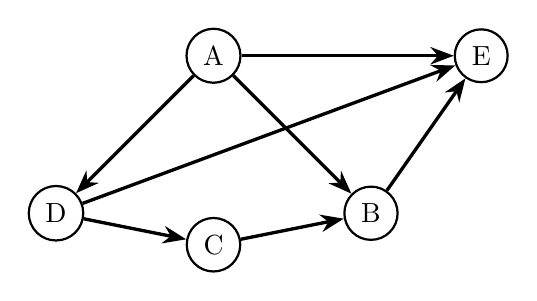
\begin{tikzpicture}
\begin{scope}[every node/.style={circle,thick,draw}]
    \node (A) at (0,0) {A};
    \node (B) at (2,-2) {B};
    \node (C) at (0,-2.4) {C};
    \node (D) at (-2,-2) {D};
    \node (E) at (3.4,0) {E};
\end{scope}

\begin{scope}[>={Stealth[black]},
              every node/.style={fill=white,circle},
              every edge/.style={draw=black,very thick}]
    \path [->] (A) edge (B);
    \path [->] (A) edge (D);
    \path [->] (A) edge (E);
    \path [->] (B) edge (E);
    \path [->] (C) edge (B);
    \path [->] (D) edge (C);
    \path [->] (D) edge (E);
\end{scope}
\end{tikzpicture}
\end{center}


\begin{parts}

\part[1] \solo Write the joint probability distribution for $P(A,B,C,D,E)$ factorized as much as possible using the conditional independence assumptions expressed by the Bayesian Network.

\begin{your_solution}[height=2cm, width=14cm]
$P(A,B,C,D,E) = P(E \big| A, B, D)P(B \big| A, C) P(C \big| D) P(D \big| A) P(A)$
\end{your_solution}


\part[1] \solo Which nodes are in the Markov boundary of $B$? Note that the Markov boundary is the smallest possible Markov blanket.

    \sall
    \begin{list}{}
        % YOUR ANSWER
        % Change \emptysquare to \filledsquare for the appropriate selection/selections 
        \item 
            %\emptysquare 
            \filledsquare
            A
            
            %\emptysquare 
            \filledsquare
            C
            
        \item 
            %\emptysquare 
            \filledsquare
            D
            
        \item 
            %\emptysquare 
            \filledsquare
            E
        \item 
            \emptysquare 
            % \filledsquare
            None of the above
    \end{list}
    
\part[1] \solo Which nodes are in the Markov boundary of $C$?

    \sall
    \begin{list}{}
        % YOUR ANSWER
        % Change \emptysquare to \filledsquare for the appropriate selection/selections 
        \item 
            %\emptysquare 
            \filledsquare
            A
            
            %\emptysquare 
            \filledsquare
            B
            
        \item 
            %\emptysquare 
            \filledsquare
            D
            
        \item 
            \emptysquare 
            % \filledsquare
            E
        \item 
            \emptysquare 
            % \filledsquare
            None of the above
    \end{list}

\clearpage

\part[1] \solo \tf $E$ is conditionally independent of $C$ given $\{A,B,D\}$. That is, \\ $E \perp C \mid \{A,B,D\}$.

    \sone
    \begin{list}{}
        % YOUR ANSWER
        % Change \emptycircle to \filledcircle for the appropriate selection/selections 
        \item 
            % \emptycircle 
            \filledcircle
            True
        \item 
            \emptycircle 
            % \filledcircle
            False
    
    \end{list}
    

\end{parts}\clearpage
\newpage
\sectionquestion{Reinforcement Learning, Revisited}
\label{sec:rl}

While attending the ML conference \textit{The Fellowship of the Ring}, you meet Elon Musk, founder of SpaceX. He has a new idea for destroying the evil lord Sauron's precious ring: fly the ring directly into the Sun. Elon has asked you to develop a reinforcement learning agent capable of carrying out the space-flight from Earth to the Sun.
You model this problem as a Markov decision process (MDP). The figure below depicts the state space. 

\begin{center}
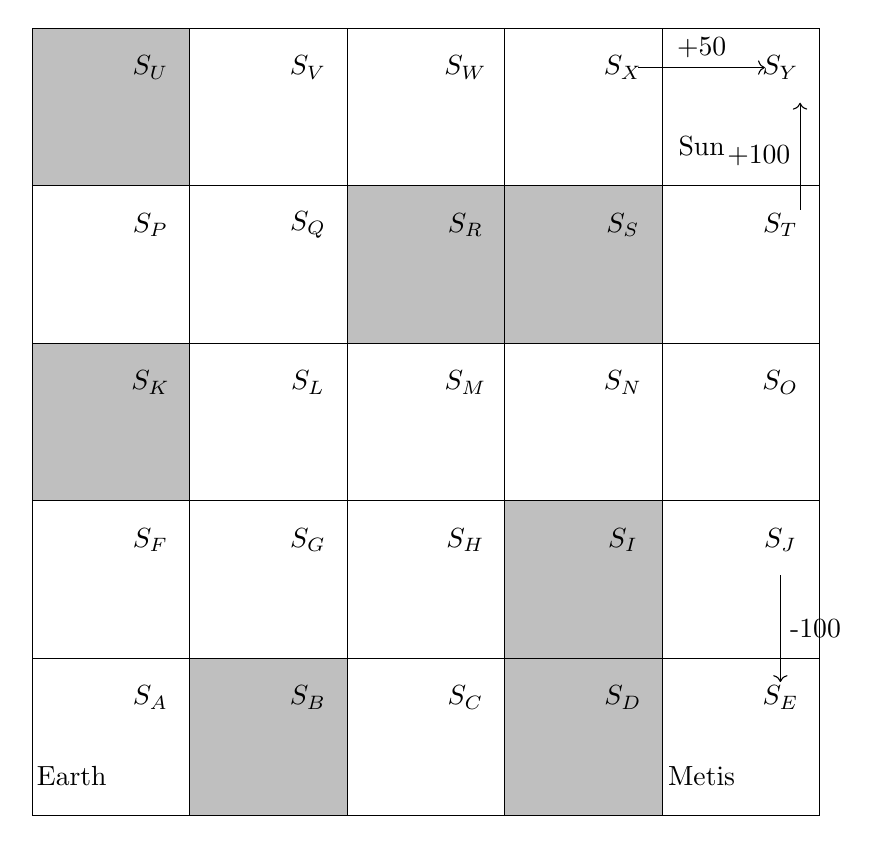
\begin{tikzpicture}
\draw[step=2cm] (0,0) grid (10, 10);

\node at (.5, 0.5) {Earth};
\node at (8.5, 8.5) {Sun};
\node at (8.5, 0.5) {Metis};

\foreach \x/\y in {
    1/0, 3/0, 3/1, 0/2, 0/4, 2/3, 3/3}
    \draw[fill=white!50!gray] 
    (2*\x,2*\y) rectangle (2*\x + 2, 2*\y + 2);


\foreach \x/\y/\m in {
    0/4/U, 1/4/V, 2/4/W, 3/4/X, 4/4/Y,
    0/3/P, 1/3/Q, 2/3/R, 3/3/S, 4/3/T,
    0/2/K, 1/2/L, 2/2/M, 3/2/N, 4/2/O,
    0/1/F, 1/1/G, 2/1/H, 3/1/I, 4/1/J,
    0/0/A, 1/0/B, 2/0/C, 3/0/D, 4/0/E}
    \node at (2*\x + 1.5,2*\y + 1.5) {$S_\m$};

\node[state, draw=none] (n1) at (7.25, 9.5) {};
\node[state, draw=none] (n2) at (9.75, 9.5) {};
\node[state, draw=none] (n3) at (9.75, 7.25) {};
\node[state, draw=none] (n4) at (9.5, 1.25) {};
\node[state, draw=none] (n5) at (9.5, 3.5) {};

\draw [->] (n1) to node[auto] { +50} (n2);
\draw [->] (n3) to node[auto] {+100} (n2);
\draw [->] (n5) to node[auto] {-100} (n4);

\end{tikzpicture}
\end{center}

Here are the details:

\begin{enumerate}
    \item Each grid cell is a state $S_A, S_B,..., S_Y$ corresponding to a position in the solar system.
    \item The action space includes movement up/down/left/right.
Transitions are deterministic. It is not possible to move into blocked states, which are shaded grey, since they contain other planets.
    \item The start state is $S_A$ (Earth). The terminal states include both the $S_Y$ (Sun) and $S_E$ (asteroid Metis, home to Sauron's cousin).
    \item Non-zero rewards are depicted with arrows.  Flying into the Sun from the left gives positive reward $R(S_X, \text{right}) = +50$. Flying into the Sun from below gives positive reward $R(S_T, \text{up}) = +100$. Flying to Metis is inadvisable and gives negative reward $R(S_J, \text{down}) = -100$. All other rewards are zero.
    \item The discount factor is $\gamma = 0.5$.
\end{enumerate}

    
Below, let $V^*(s)$ denote the value function for state $s$ using the optimal policy $\pi^*(s)$. Let $Q^*(s,a)$ denote the Q function for $\pi^*$.

\clearpage

\begin{parts}

\part[1] \solo What is the value $V^*(S_T)$?

\begin{your_solution}[height=2cm, width=4cm]
$100$
\end{your_solution}


\part[1] \solo What is the value $V^*(S_O)$?

\begin{your_solution}[height=2cm, width=4cm]
$50$
\end{your_solution}


\part[1] \solo What is the value $V^*(S_A)$?

\begin{your_solution}[height=2cm, width=4cm]
$0.78125$
\end{your_solution}


\part[1] \solo What is the value $Q^*(S_T, \text{up})$?

\begin{your_solution}[height=2cm, width=4cm]
$100$
\end{your_solution}


\part[1] \solo What is the value $Q^*(S_T, \text{down})$?

\begin{your_solution}[height=2cm, width=4cm]
$25$
\end{your_solution}


\part[1] \solo What action does the optimal policy take from state $S_Q$ (i.e. what is $\pi^*(S_Q)$)? (Note: If the optimal policy is not unique and there are multiple optimal actions, select them all.)

    \sall
    \begin{list}{}
        % YOUR ANSWER
        % Change \emptysquare to \filledsquare for the appropriate selection/selections 
        \item 
            % \emptysquare 
            \filledsquare
            Up
            
            \emptysquare 
            % \filledsquare
            Down
            
        \item 
            \emptysquare 
            % \filledsquare
            Left
            
        \item 
            \emptysquare 
            % \filledsquare
            Right
    \end{list}
    
\clearpage

Now suppose you employ Q-Learning to learn table values $Q(s,a)$ for each state $s$ and action $a$. The table is initialized to all zeros. On the very first episode of training, you begin at state $S_A$ (Earth), take eight steps, and arrive in state $S_E$ (Metis). At each step, you perform a Q-Learning update of the appropriate entry in $Q(s,a)$. Assume a learning rate $\alpha=1$.

\part[1] \solo What is the new table value found in $Q(S_J,\text{down})$ after this episode?

\begin{your_solution}[height=2cm, width=4cm]
$-100$
\end{your_solution}


\part[1] \solo What is the new table value found in $Q(S_O,\text{down})$ after this episode?

\begin{your_solution}[height=2cm, width=4cm]
$0$
\end{your_solution}



\part[1] \solo \tf The Q-function is guaranteed to converge to the true Q-values in this environment given the specified initialization and assuming that the Q-Learning algorithm visits each state-action pair infinitely often.

    \sone
    \begin{list}{}
        % YOUR ANSWER
        % Change \emptycircle to \filledcircle for the appropriate selection/selections 
        \item 
            %\emptycircle 
            \filledcircle
            True
            % True in this setting for detereministic transitions. Plus, finite
        \item 
            \emptycircle 
            % \filledcircle
            False
    
    \end{list}
    

\end{parts}\clearpage
\newpage
\sectionquestion{PCA}
\label{sec:pca}

\begin{parts}
    
    \fullwidth{\textbf{{\large Some PCA Theory}}}
    
    \part[2] \solo Assume we apply PCA to a matrix $X \in R^{n \times m}$ and obtain a set of PCA features, $Z \in R^{n \times m}$ .We divide this set into two, $Z1$ and $Z2$. The first set, Z1, corresponds to the top principal components. The second set, Z2, corresponds to the remaining principal components. Which is more common in the training data:
    
    \sone
    \begin{list}{}
        % YOUR ANSWER
        % Change \emptycircle to \filledcircle for the appropriate selection/selections 
        \item 
            %\emptycircle 
            \filledcircle
            a point with large feature values in $Z1$ and small feature values in  $Z2$
        \item 
            \emptycircle 
            % \filledcircle
            a point with large feature values in $Z2$ and small feature values in  $Z1$
        \item 
            \emptycircle 
            % \filledcircle
            a point with large feature values in $Z2$ and large feature values in  $Z1$
        \item 
            \emptycircle 
            % \filledcircle
            a point with small feature values in $Z2$ and small feature values in  $Z1$
    \end{list}
    
    
    
    \part[1] \solo For the data set shown below, assume the data are centered at the \textbf{origin}. Further, refer to the x-axis as component 1, and the y-axis as component 2. What is its first principal component, if it exists? 
    \begin{figure}[H]
    \centering
    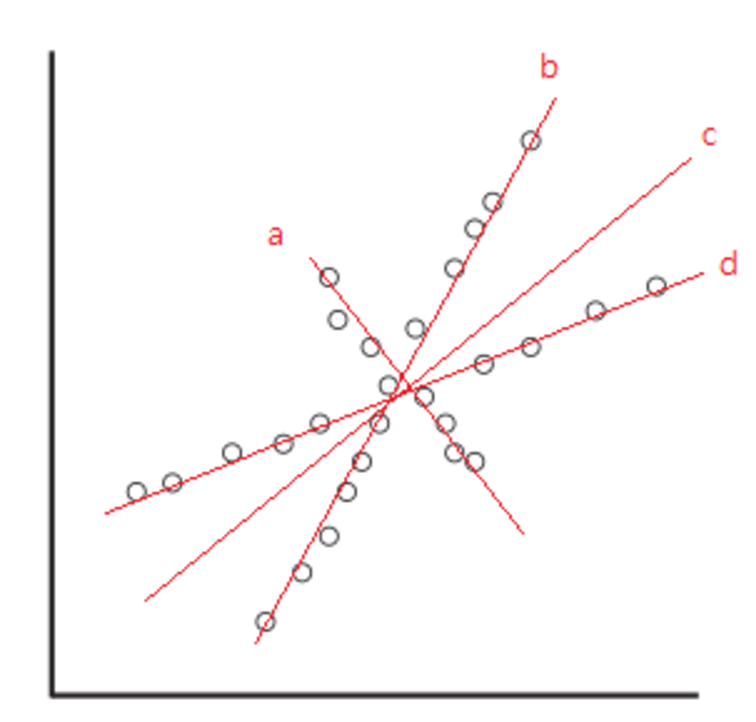
\includegraphics[width=0.65\linewidth]{figures/pca1.png}
    \end{figure}
    \newpage

    \sone
    \begin{list}{}
        % YOUR ANSWER
        % Change \emptycircle to \filledcircle for the appropriate selection/selections 
        \item 
            \emptycircle 
            % \filledcircle
            a
        \item 
            \emptycircle 
            %\filledcircle
            b
        \item 
            % \emptycircle 
            \filledcircle
            c
            % Projection onto C
        \item 
            \emptycircle 
            % \filledcircle
            d
        \item 
            \emptycircle 
            % \filledcircle
            None of the above
    \end{list}
    
    
    \part[1] \solo \textbf{NOTE : This is continued from the previous question.} What is the second principal component in the figure from the previous question, if it exists? 

    \sone
    \begin{list}{}
        % YOUR ANSWER
        % Change \emptycircle to \filledcircle for the appropriate selection/selections 
        \item 
            % \emptycircle 
            \filledcircle
            a
        \item 
            \emptycircle 
            % \filledcircle
            b
        \item 
            \emptycircle 
            % \filledcircle
            c
        \item 
            \emptycircle 
            % \filledcircle
            d
        \item 
            \emptycircle 
            % \filledcircle
            None of the above
    \end{list}
    

    \part[1] \solo \textbf{NOTE : This is continued from the previous question.} What is the third principal component in the figure from the previous question, if it exists?

    \sone
    \begin{list}{}
        % YOUR ANSWER
        % Change \emptycircle to \filledcircle for the appropriate selection/selections 
        \item 
            \emptycircle 
            %\filledcircle
            a
        \item 
            \emptycircle 
            % \filledcircle
            b
        \item 
            \emptycircle 
            % \filledcircle
            c
        \item 
            \emptycircle 
            % \filledcircle
            d
        \item 
            % \emptycircle 
            \filledcircle
            None of the above
    \end{list}
    

    \vspace{1cm}
    
\clearpage

    \fullwidth{\textbf{{\large PCA in Practice}}}
    
    \uplevel{
    For this section, refer to the PCA demo linked \href{https://colab.research.google.com/drive/1yOKqauw5XiVJCDJgQh4UZtkA2AOjXLRG?usp=sharing}{here}. In this demonstration, we have performed PCA for you on a \href{https://en.wikipedia.org/wiki/Iris_flower_data_set}{simple four-feature dataset}. The questions below have also been added to the colab notebook linked for ease of access. Run the code in the notebook, then answer the questions based on the results. Once you've answered the following questions, feel free to make a copy of the notebook to further explore how PCA works. 
    }
    
    \part[2] \group We begin by normalizing each of the columns in our data (ie: adjusting the data to be between 0 and 1, here implemented through \href{https://towardsdatascience.com/everything-you-need-to-know-about-min-max-normalization-in-python-b79592732b79}{min-max scaling}. Why is this a good idea? Additionally, why is it potentially a bad idea to standardize our features (ie: adjust all the features to have a variance of 1)?
    
    \begin{your_solution}[height=4cm, width=0.95\textwidth]
    % to bring everything to same scale else feature comparison wont be effective.
    % variance cant be limited as you want your pc to capture the data spread details.
    \vspace{-5pt}
    PCA tries to capture the direction in which the variance is maximized. The higher the variance captured, the better that component is able to represent the data distribution. However, if the features have different scales, their variances will not be a true representation of their importance in capturing the data distribution. Hence, it's preferred to normalize the features. Similarly, you wouldn't want to standardize the features as that would lead to all having a variance of 1. If all features have a variance 1 then, PCA would be incorrect as the data representation would be affected due to standardization.`
    \end{your_solution}
    
    \part[2] \group  Below this question (in the \href{https://colab.research.google.com/drive/1yOKqauw5XiVJCDJgQh4UZtkA2AOjXLRG?usp=sharing}{colab} file), we plot each of the features against each other. Do you see any special relationships between any of the features? In particular, take a look at the \texttt{petal\_length} feature. How would you describe its association with each of the other features? Note: there is no need to copy the plots to your submission.
    
    \begin{your_solution}[height=4cm, width=0.95\textwidth]
    Some of the feature pairs are successfully able to group the data properly. n particular, \texttt{petal\_length}. \texttt{petal\_length} with each of the other features is able to successfully capture most of the distribution information. Especially, \texttt{petal\_length}  and \texttt{petal\_width}. The corresponding plot shows that these 2 features are able to represent the data of 3 classes with minimal overlap based on the plot.
    \end{your_solution}
    
    \part[2] \group To get the principal components of the features, we will calculate the eigenvalues and eigenvectors of the covariance matrix. If we took the dot product of any two eigenvectors, what should it be? What does it mean to obtain this value and why is this property beneficial?
    
    \begin{your_solution}[height=4cm, width=0.95\textwidth]
    % 0, they're orthogonal, that the eigen vectors or PCs are uncorrelated and thus, there's no redundancy in the feature information that they capture/represent
    The dot product of any 2 eigen vectors should be 0. This means that an eigen vector is orthogonal to other eigen vectors. This property ensures that the eigen vectors or principal components are uncorrelated and thus, there's no redundancy in the feature information they capture or represent. The principal components independently represent certain data characteristics.
    \end{your_solution}
    
    \part[2] \group If we wanted to find $k$ principal components such that we preserve \textbf{at least} 95\% of the variance in the data, what would be the value of $k$? Hint: it is helpful here to look at the cumulative variance in the first $k$ components, which we have calculated for you.
    
    \begin{your_solution}[height=2.5cm, width=4cm]
    2
    \end{your_solution}
    
    \part[2] \group Taking note of the principal components plot, let's take a look back at the scatter matrix. If we wanted to perform dimensionality reduction to have just two features, we could pick any two features from the dataset, and train a classifier on just those. What is one reason we could prefer the PCA features to just choosing two of the original features to represent our data?
    
    \begin{your_solution}[height=4cm, width=0.95\textwidth]
    The distribution as per the principal components has a greater variance and thus, captures the spread of the data much better than that by any 2 of the normalized features. Principal components are formed Thus, it would lead to fewer misclassifications on the test set as compared to that using 2 features.
    \end{your_solution}
    
\end{parts}\clearpage
\newpage
\titledquestion{K-Means}
\label{sec:kmeans}

 \begin{figure}[H]
        \begin{center}
        \begin{subfigure}{.6\textwidth}
             %\centering
            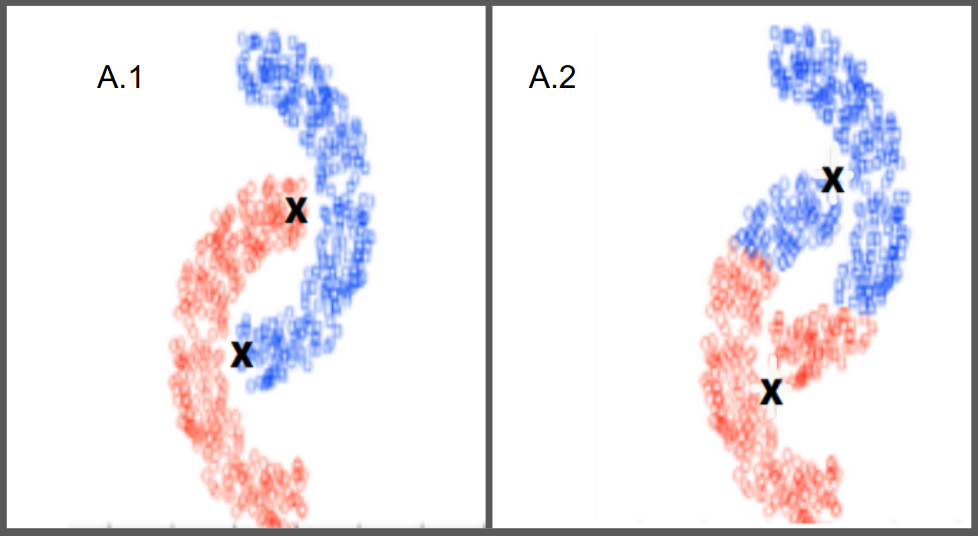
\includegraphics[width=\linewidth]{figures/d12.png}
        %%        %\centering
            \caption{Dataset A}
            \label{fig:sfig1}
        \end{subfigure}
        %\end{center}
        %\begin{center}
        \begin{subfigure}{.6\textwidth}
             %\centering
            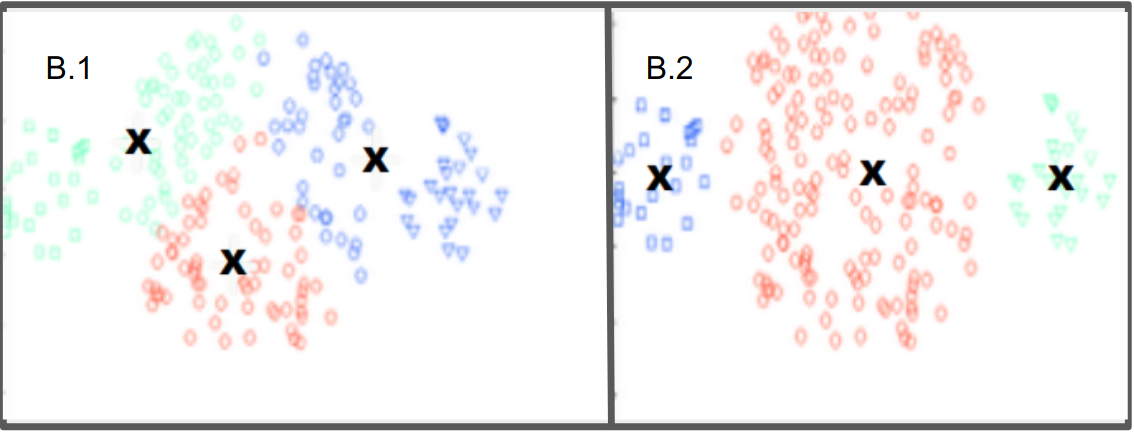
\includegraphics[width=\linewidth]{figures/d23.png}
        %    %\centering
            \caption{Dataset B}
            \label{fig:sfig2}
        \end{subfigure}
        \end{center}

        \begin{center}
        \begin{subfigure}{.6\textwidth}
            %\centering
            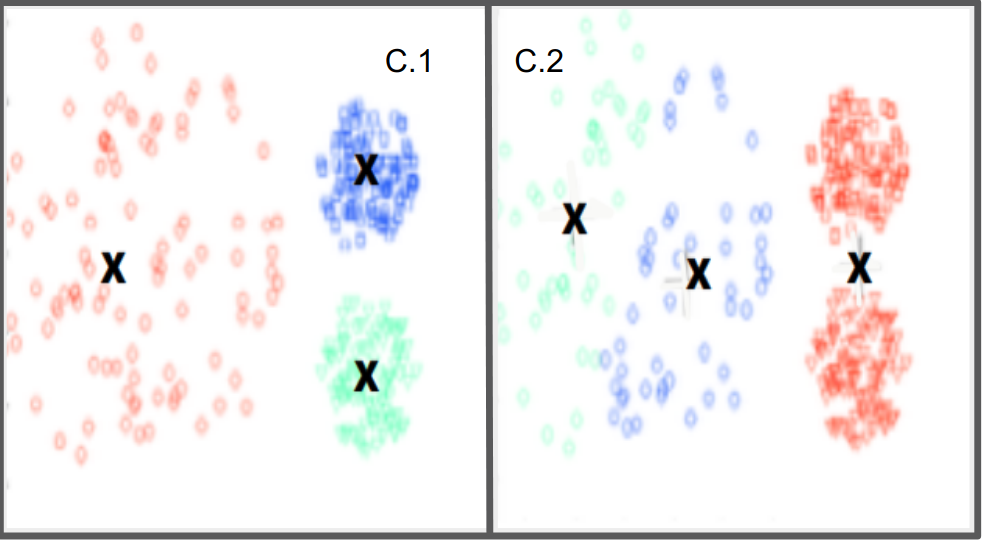
\includegraphics[width=\linewidth]{figures/d32.png}
            %\centering
            \caption{Dataset C}
            \label{fig:sfig3}
        \end{subfigure}   
        \end{center}
     % \end{tabular}
     
     
         \caption{Datasets}
          \label{fig:KMeans}
       
         %\caption{4 x 4}
        %\end{figure}
        \end{figure}

\newpage

\begin{parts}

\part
Consider the 3 datasets A, B and C as shown in Figure~\ref{fig:KMeans}. Each dataset is classified into $k$ clusters as represented by different colors in the figure. For each dataset, select the image with cluster centers (denoted by an X) that is generated by K-means. The distance measure used here is the Euclidean distance.
\begin{subparts}
 \subpart[1] \solo Dataset A $\textbf{(Select one)}$
 \begin{list}{}
        \item $\circle$ A.1
        \item $\CIRCLE$ A.2
    \end{list}

    
 \subpart[1] \solo Dataset B $\textbf{(Select one)}$
 \begin{list}{}
        \item $\CIRCLE$ B.1
        \item $\circle$ B.2
    \end{list}

 
 \subpart[1] \solo Dataset C $\textbf{(Select one)}$
 \begin{list}{}
        \item $\circle$ C.1
        \item $\CIRCLE$ C.2
    \end{list} 
 
\end{subparts}

%\clearpage
 \part Consider a Dataset $\mathcal{D}$ with 5 points as shown below. Perform a K-means clustering on this dataset with $k=2$ using the Euclidean distance as the distance function.
 Remember that in the K-means algorithm, an iteration consists of performing following tasks: Assigning each data point to it's nearest cluster center followed by recomputating those centers by taking an average based on all the data points assigned to it. Initially, the 2 cluster centers are chosen randomly as $\mu0$ = (5.3, 3.5), $\mu1$ = (5.1, 4.2). Parts (a) through (d) refer only to the first iteration of K-means clustering performed on $\mathcal{D}$.
 
\[
\mathcal{D}=\begin{bmatrix}
5.5&3.1\\
5.1&4.8\\
6.6&3.0\\
5.5&4.6\\
6.8&3.8\\
%5.5&3.1\\
% 6.9&3.4\\
% 5.5&4.6\\
% 6.3&4.9\\
% 5.5&3.9\\
\end{bmatrix}
\]

    \begin{subparts}
    \subpart[2] \solo Which of the following points will be the center for cluster 0?
    \textbf{Select one:}
    \begin{list}{}
        \item $\circle$ (5.7 , 4.1)
        \item $\circle$ (5.6 , 4.8)
        \item $\CIRCLE$ (6.3 , 3.3)
        \item $\circle$ (6.7 , 3.4)
    \end{list}


    \newpage
    \subpart[2] \solo Which of the following points will be the center for cluster 1?
    \textbf{Select one:}
    \begin{list}{}
        \item $\circle$ (6.1 , 3.8)
        \item $\circle$ (5.5 , 4.6)
        \item $\circle$ (5.4 , 4.7)
        \item $\CIRCLE$ (5.3 , 4.7)
    \end{list}


    
    \subpart[1] \solo How many points will belong to cluster 0?
    
    
    \begin{your_solution}[title=Answer, height=2cm, width=3cm]
    3
    \end{your_solution}


    
    \subpart[1] \solo How many points will belong to cluster 1?
    
    
    \begin{your_solution}[title=Answer, height=2cm, width=3cm]
	2    
    \end{your_solution}
    


   \end{subparts}
   
   \part Recall that in K-means clustering we attempt to find $k$ cluster centers $c_j \in \R^d$ (where $d$ is the dimension of the data), $j\in \{1,\dots,k\}$ such that the total distance between each datapoint and the nearest cluster center is minimized. Then the objective function is,
   \begin{align}
   \sum_{i=1}^n \min_{j\in\{1,\dots ,k\}} ||x_i - c_j||^2 
   \label{eq:kmeansObj}
   \end{align}
   In other words, we attempt to find $c_1 ,\dots ,c_k$ that minimizes Eq. \eqref{eq:kmeansObj}, where n is the number of data points. To do so, we iterate between assigning $x_i$ to the nearest cluster center and updating each cluster center $c_j$ to the average of all points assigned to the $j^{\textrm{th}}$ cluster.  Instead of holding the number of clusters $k$ fixed, your friend John tries to minimize Eq. \eqref{eq:kmeansObj} over $k$. Yet, you found this idea to be a bad one. 

    Specifically, you convinced John by providing two values $\alpha$, the minimum possible value of Eq. \eqref{eq:kmeansObj}, and $\beta$, the value of $k$ when Eq. \eqref{eq:kmeansObj} is minimized. 

    \begin{subparts}
    \subpart[1] \solo What is the value of $\alpha$ when $n=100$?

    \begin{your_solution}[title=Answer, height=2cm, width=3cm]
    0
    % essentially, k = 100 and so, each point is it's own cluster center.
    \end{your_solution}
    
    
    \subpart[1] \solo What is the minimum value of $\beta$ when $n=100$?

    \begin{your_solution}[title=Answer, height=2cm, width=3cm]
    100
    \end{your_solution}
    

    \subpart[2] \solo We want to see how K-means clustering works on a single dimension. Consider the case in which $k = 3$ and we have 4 data points $x_1=1, x_2 = 2, x_3 = 5, x_4 =7$. What is the optimal value of the objective Eq. \eqref{eq:kmeansObj} when $k$ is fixed at $3$? 
    
    \begin{your_solution}[title=Answer, height=2cm, width=3cm]
    0.5
    % 5, 7, 1.5/1/2 - squared 
    \end{your_solution}

    

    \end{subparts}
    
    \clearpage
    
    \part[3] \group Consider the following simple brute-force algorithm for minimizing the K-means objective:
    \begin{enumerate}
        \item Enumerate all the possible partitionings of the $n$ points into $k$ clusters. 
        \item For each possible partitioning, compute the optimal centers $c_1 , . . . , c_k$ by taking the mean of the points in each cluster and compute the corresponding K-means objective value.
        \item Output the best clustering found.
    \end{enumerate}
    
      This algorithm is guaranteed to output the optimal set of centers, but unfortunately its running time is exponential in the number of data points. For the case $k = 2$, justify that the running time of the brute-force algorithm above is exponential in the number of data points $n$.
    
   \begin{your_solution}[height=3cm, width=.95\textwidth]
   \vspace{-5pt}
   Each of the $n$ points could belong to either of the 2 clusters. Thus, $x^{(1)}$ can take 2 values, $x^{(2)}$ can take 2 values and similarly, $x^{(n)}$ can take 2 values. Thus, the number of combinations/partitionings possible would be $2^n$ and similary, the corresponding runtime of the algorithm would be $\mathbb{O}(n2^n)$. Thus, as $n$ increases, the runtime increases exponentially.
    \end{your_solution}

    
    \part Initializing the centers has a big impact on the performance of Lloyd's clustering algorithm. Usually, we randomly initialize $k$ cluster centers. However, there are other methods, namely, furthest point initialization and $k$-means++ initialization.
    
    \begin{subparts}
    \subpart[2] \group Essentially, in $k$-means++, the first cluster center is chosen uniformly at random from the data points, after which each subsequent cluster center is chosen from the remaining (not chosen) data points. The probability of each point to be chosen as the next center is proportional to the squared distance to closest existing cluster center.
    
    \begin{figure}[H]
        \centering
        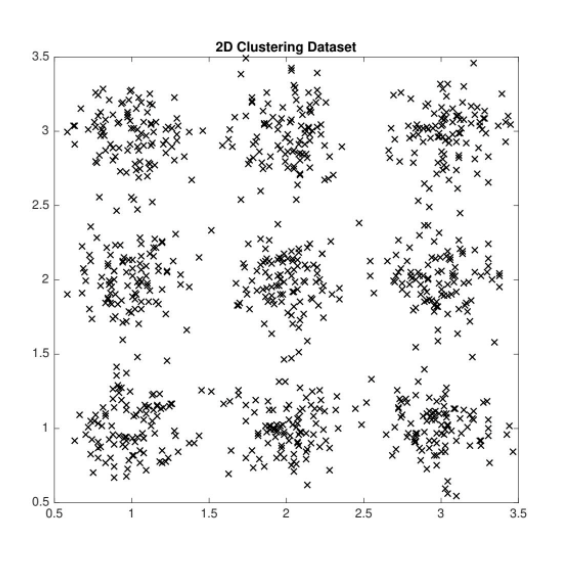
\includegraphics[width=0.5\linewidth]{figures/kmeans.png}
        \caption{2D Dataset}
        \label{fig:KMeans2}
    \end{figure}
    
    Explain in 1– 2 sentences why using  $k$-means++ initialization is more likely to choose one sample from each cluster than random initialization from the dataset in Figure 2 above. Recall that random initialization is randomly choosing a set of data points as starting cluster centers. 
    
    \begin{your_solution}[height=3cm, width=.95\textwidth]
    \vspace{-5pt}
    Say, the first center ($c_1$) is chosen from the top-left set of points. However, the subsequent center has a higher probability of being chosen from the set of points furthest from $c_1$. So, $c_2$ would be somewhere near the bottom right. Similarly, all subsequent centers would be chosen with high probability from a set of points away from centers leading to a center in every separate cluster. For example, $c_3$, $c_4$ have a higher chance of being along the other diagonal.
    \end{your_solution}

    
    \subpart[2] \group
    Another method of initialization is furthest point initialization. Essentially, the first cluster center is chosen at random. Then, pick the rest of the cluster centers, one by one, among the datapoints that are the furthest from the cluster centers chosen thus far. 
    
    Given this definition, is the furthest point initialization sensitive to outliers? Explain why or why not.
    
    \begin{your_solution}[height=3cm, width=.95\textwidth]
    \vspace{-5pt}
    Yes, this would be sensitive to outliers. Consider points distributed within 2 circles of radius 1 close to each other and 1 outlier at a distance of 5 from their centers. The $1^{st}$ center has a high probability of being assigned to one of the points within the circles. However, the $2^{nd}$ center would be the outlier. Now, k-means would converge to the outlier being one cluster and the two circles being another whereas the ideal clustering would have separated the 2 circles.
    \end{your_solution}

    \end{subparts}

\end{parts}
\clearpage
\newpage
\sectionquestion{Ensemble Methods}
\label{sec:ensemble}

\begin{parts}
\part[1] \solo 
    Which of the following is false?
    
        \sone
        \begin{list}{}
        % YOUR ANSWER
        % Change \emptycircle to \filledcircle for the appropriate selection/selections 
        \item 
            \emptycircle 
            % \filledcircle
            In the weighted majority algorithm, the weights associated with the weak learners are learned during training.
        \item 
            %\emptycircle 
            % \filledcircle
            In the AdaBoost algorithm, the weights associated with the weak learners are learned during training.
        \item 
            % \emptycircle 
            \filledcircle
            In the weighted majority algorithm, the weak learners are learned during training.
        \item 
            \emptycircle 
            % \filledcircle
            In the AdaBoost algorithm, the weak learners are learned during training.
    \end{list}
    

\part[1] \solo \tf Provided enough iterations are performed, AdaBoost will give zero training error on any dataset regardless of the type of weak learner used.

    \sone
    \begin{list}{}
        % YOUR ANSWER
        % Change \emptycircle to \filledcircle for the appropriate selection/selections 
        \item 
            % \emptycircle 
            \filledcircle
            True
        \item 
            \emptycircle 
            % \filledcircle
            False
    
    \end{list}
    
    
\part[1] \solo \tf Consider some training point $(x_i, y_i)$ to the AdaBoost algorithm. If all weak learners during training correctly classify $x_i$ as label $y_i$, there will eventually be a time $t$ such that the weight assigned to $x_i$ in the training distribution $\D_t$ reaches $0$.

    \sone
    \begin{list}{}
        % YOUR ANSWER
        % Change \emptycircle to \filledcircle for the appropriate selection/selections 
        \item 
            \emptycircle 
            % \filledcircle
            True
        \item 
            % \emptycircle 
            \filledcircle
            False
    
    \end{list}
    

\part[1] \solo \tf If AdaBoost reaches perfect training accuracy, all weak learners created in subsequent iterations will be identical.

    \sone
    \begin{list}{}
        % YOUR ANSWER
        % Change \emptycircle to \filledcircle for the appropriate selection/selections 
        \item 
            \emptycircle 
            % \filledcircle
            True
        \item 
            % \emptycircle 
            \filledcircle
            False
    
    \end{list}
    

\clearpage

\part[1] \solo Consider the following table containing recorded weights from iterations of AdaBoost. Which of the training points (A, B, C, D, E, F) must have been misclassified in Round 220 in order to produce the updated weights shown at the start of Round 221?

\begin{center}
\begin{tabular}{ |c|c|c|c|c|c|c| } 
 \hline
 Round & $D_t(A)$ & $D_t(B)$ & $D_t(C)$ & $D_t(D)$ & $D_t(E)$ & $D_t(F)$ \\ [4pt]
  \hline
  \hline
\multicolumn{7}{|c|}{...}\\[4pt]
  \hline 220 & $\frac{1}{14}$ & $\frac{1}{14}$ & $\frac{7}{14}$ & $\frac{1}{14}$ & $\frac{2}{14}$ & $\frac{2}{14}$ \\ [4pt]
   \hline
 221 & $\frac{5}{40}$ & $\frac{5}{40}$ & $\frac{14}{40}$ & $\frac{2}{40}$ & $\frac{10}{40}$ & $\frac{4}{40}$ \\ [4pt]
 \hline
 \multicolumn{7}{|c|}{...}\\[4pt]
   \hline
\end{tabular}
\end{center}

    
    \sall
    \begin{list}{}
        % YOUR ANSWER
        % Change \emptysquare to \filledsquare for the appropriate selection/selections 
        \item 
            % \emptysquare 
            \filledsquare
            A
            
            % \emptysquare 
            \filledsquare
            B
            
        \item 
            \emptysquare 
            % \filledsquare
            C
            
        \item 
            \emptysquare 
            % \filledsquare
            D
        \item 
            % \emptysquare 
            \filledsquare
            E
        \item 
            \emptysquare 
            % \filledsquare
            F
    \end{list}

\clearpage

\part
In the following question, we will examine the generalization error of AdaBoost using a concept known as the \textit{classification margin}.

Throughout the question, use the following definitions:
\begin{itemize}
    \item $T$: The number of iterations used to train AdaBoost.
    \item $N$: The number of training samples.
    \item $S = \{(x_1, y_1), \cdots, (x_N, y_N)\}$: 
        The training samples with binary labels ($\forall i \in [N] \ y_i \in \{-1, +1\}$).
    \item $d$: The VC-dimension of the weak learner hypothesis class.
    \item $\D_t (i)$: The weight assigned to training example $i$ at time $t$.
        Note that $\sum_i \D_t (i) = 1$.
    \item $h_t$: The weak learner constructed at time $t$.
    \item $\epsilon_t$: The error of $h_t$ on $\D_t$.
    \item $Z_t = 2\sqrt{\epsilon_t (1 - \epsilon_t)}$: The normalization factor for the distribution update at time $t$.
    \item $\alpha_t = \frac{1}{2} \ln ((1 - \epsilon_t)/\epsilon_t)$: The weight assigned to the learner $h_t$ in the composite hypothesis.
    \item $f_t (x) = \left( \sum_{t'=1}^{t} \alpha_{t'} h_{t'} (x) \right) / \left( \sum_{t'=1}^{t} \alpha_{t'} \right)$: 
        The majority vote of the weak learners, rescaled based on the total weights.
    \item $H_{t} (x) = \sign(f_{t} (x))$: The voting classifier decision function.
    \item $\trainerr{H}$: The training error of classifier $H$.
    \item $\generr{H}$: The generalization error of classifier $H$.
\end{itemize}

Consider a binary classification task where our classifier generates a distribution of weights, or confidence scores, over the possible labels.
To form a valid distribution, such weights must fall into the range $[0, 1]$ and must sum to $1$.
The classifier output is the label which has the largest associated weight.
We define the \textit{classification margin} for an input as the difference between the weight assigned to the correct label and the incorrect label.

\begin{subparts}
\subpart[1] \group What is the range of values the classification margin can take on?

\begin{your_solution}[height=3cm, width=6cm]
$[-1, 1]$
\end{your_solution}


\clearpage

\subpart[1] \group Let $\margin_t (x, y)$ represent the margin for our AdaBoost classifier at iteration $t$ on the sample $(x, y)$. Write a single inequality in terms of $\margin_t (x, y)$ that is true if and only if the classifier makes a mistake on the input $(x, y)$ (i.e., provide a bound on the margin in the case the classifier is incorrect). Assume the classifier makes a mistake on ties.


\begin{your_solution}[height=3cm, width=6cm]
\end{your_solution}



\subpart[1] \group For a given input and label $(x_i, y_i)$, write $\margin_t (x_i, y_i)$ in terms of $x_i, y_i$ and $f_t$.

\begin{your_solution}[height=3cm, width=6cm]
\end{your_solution}

\subpart[1] \group Recall the update AdaBoost performs on the distribution of weights:
\begin{itemize}
    \item $\D_1 (i) = 1 / N$
    \item $\D_{t+1} (i) = \D_t (i) \dfrac{\exp(-y_i \alpha_t h_t (x_i))}{Z_t}$.
\end{itemize}
Fill in the blank for the following expression for $\D_{t+1} (i)$. You may use $x_i, y_i$, and both of $\alpha, h$ at any iteration in your answer.
$$ \D_{t+1} (i) = \dfrac{1}{N} \left( \prod_{t'=1}^t \dfrac{1}{Z_{t'}} \right) \exp ( \underline{\hspace{2cm}} )$$

\begin{your_solution}[height=3cm, width=6cm]
$-y_i \sum \limits_{t' =  1}^t \alpha_{t'}h_{t'}(x_i)$
\end{your_solution}

\clearpage

\subpart[1] \group Let $\alpha = \sum_{t'=1}^t \alpha_{t'}$. Rewrite your above answer in terms of $y_i, \alpha, f_t, x_i$.

\begin{your_solution}[height=3cm, width=6cm]
$-y_i \alpha f_{t}(x_i)$
\end{your_solution}



\subpart[1] \group Rewrite your above answer in terms of $\margin_t (x_i, y_i)$ and $\alpha$.

\begin{your_solution}[height=3cm, width=6cm]
\end{your_solution}



\subpart[1] \group Note that $\alpha$ is constant across the input points. Using the classification margin, describe which points AdaBoost assigns high weight to at time $t$.

\begin{your_solution}[height=3cm, width=.9\textwidth]
\end{your_solution}



\uplevel{
Consider $\PrSinline \left[\margin_{T} (x_i, y_i) \leq \theta \right]$, the fraction of inputs with margin below a margin threshold $\theta > 0$ for the combined hypothesis. Suppose we are able to find weak learners below $1/2$ error at all time steps. As a result of the weighting behavior you discovered in the above parts, AdaBoost decreases $\PrSinline \left[\margin_{T} (x_i, y_i) \leq \theta \right]$ exponentially fast in the number of iterations $T$.

Now, consider the following high-probability bounds on the generalization (true) error of AdaBoost.
The first bound stems from a traditional PAC learning analysis, while the second stems from a classification margin analysis.
\begin{align*}
     \text{Bound 1}: &\generr{H_T} \leq \trainerr{H_T} + 
        O \left( \sqrt{T \log T} \sqrt{d} \sqrt{\frac{\log N}{N}} \right) \\
     \text{Bound 2}: &\generr{H_T} \leq \PrS \left[\margin_T (x_i, y_i) \leq \theta \right] +
        O \left( \frac{1}{\theta} \sqrt{d} \sqrt{\frac{\log^2 N}{N}} \right)
\end{align*}
}

\clearpage

\subpart Suppose we have achieved $\trainerr{H} = 0$. Considering only the first bound, and supposing we want as tight a bound on true error as possible, should we continue training? Why or why not?

\begin{subsubparts}
    \subsubpart[1] \group
    \sone
    \begin{list}{}
        % YOUR ANSWER
        % Change \emptycircle to \filledcircle for the appropriate selection/selections 
        \item 
            \emptycircle 
            % \filledcircle
            Continue training
        \item 
            \emptycircle 
            % \filledcircle
            Stop training
    
    \end{list}
    
    
    \subsubpart[1] \group Justify your selection:
    
    \begin{your_solution}[title=Justification,height=3cm, width=.85\textwidth]
    \end{your_solution}
    

\end{subsubparts}





\subpart Suppose we have achieved $\trainerr{H} = 0$. Considering only the second bound, and supposing we want as tight a bound on true error as possible, should we continue training? Why or why not?

\begin{subsubparts}
    \subsubpart[1] \group
    \sone
    \begin{list}{}
        % YOUR ANSWER
        % Change \emptycircle to \filledcircle for the appropriate selection/selections 
        \item 
            \emptycircle 
            % \filledcircle
            Continue training
        \item 
            \emptycircle 
            % \filledcircle
            Stop training
    
    \end{list}
    
    
    \subsubpart[1] \group Justify your selection:
    
    \begin{your_solution}[title=Justification,height=3cm, width=.85\textwidth]
    \end{your_solution}



\end{subsubparts}


\subpart[1] \group \tf Considering both bounds, it is reasonable to stop training AdaBoost as soon as $\trainerr{H} = 0$.

    \sone
    \begin{list}{}
        % YOUR ANSWER
        % Change \emptycircle to \filledcircle for the appropriate selection/selections 
        \item 
            \emptycircle 
            % \filledcircle
            True
        \item 
            \emptycircle 
            % \filledcircle
            False
    
    \end{list}


\end{subparts}

\end{parts}
\clearpage
\newpage
\sectionquestion{Recommender Systems}
\label{sec:recsys}

\begin{parts}

 \part[2] \solo In which of the following situations will a collaborative filtering system be more appropriate learning algorithm compared to linear or logistic regression?
    
    \textbf{Select all that apply:}
    
        \begin{list}{}
        \item $\blacksquare$ You manage an online bookstore and you have the book ratings from many users. For each user, you want to recommend other books she will enjoy, based on her own ratings and the ratings of other users.
        \item $\blacksquare$ You run an online news aggregator, and for every user, you know some subset of articles that the user likes and some different subset that the user dislikes. You'd want to use this to find other articles that the user likes.
        \item $\square$ You've written a piece of software that has downloaded news articles from many news websites. In your system, you also keep track of which articles you personally like vs. dislike, and the system also stores away features of these articles (e.g., word counts, name of author). Using this information, you want to build a system to try to find additional new articles that you personally will like.
        \item $\square$ You manage an online bookstore and you have the book ratings from many users. You want to learn to predict the expected sales volume (number of books sold) as a function of the average rating of a book.
        \item $\square$ None of the above
    \end{list}

    
 

 \part[2] \solo What is the basic intuition behind matrix factorization?
    
    \textbf{Select all that apply:}
    
        \begin{list}{}
        \item $\square$ That content filtering and collaborative filtering are just two different factorizations of the same rating matrix.
        \item $\square$ That factoring user and item matrices can partition the users and items into clusters that can be treated identically, reducing the complexity of making recommendations.
        \item $\square$ The user-user and item-item correlations are more efficiently computed by factoring matrices.
        \item $\blacksquare$ That user-item relations can be well described in a low dimensional space that can be computed from the rating matrices.
        \item $\square$ None of the above
    \end{list}
    
    
    
    \clearpage
    
    \newpage
    \part To plan your schedule for next semester, you decide to use the recommender system by checking the courses your 10-601 TAs have taken. The course chart below shows everyone's course status. For entry values, 1 indicates that the course has been taken and 0 indicates that the course has not been taken yet.
    \begin{center}
        \begin{tabular}{|c|c|c|c|c|c|c|c|c|}
            \hline
             & 15122 & 15150 & 15210 & 15213 & 10301 & 10403 & 10725 & 11344 \\
            \hline
            \textbf{You} & 1 & 1 & 0 & 0 & 1 & 0 & 0 & 0 \\
            \hline
            Abhi & 1 & 1 & 1 & 0 & 1 & 1 & 1 & 1 \\
            \hline
            Chi & 1 & 0 & 0 & 1 & 1 & 0 & 0 & 0 \\
            \hline
            Helena & 1 & 1 & 0 & 0 & 1 & 1 & 0 & 1 \\
            \hline
            Sana & 1 & 1 & 0 & 0 & 1 & 1 & 1 & 1 \\
            \hline
            Sami & 1 & 1 & 1 & 1 & 1 & 1 & 0 & 0 \\
            \hline
        \end{tabular}
    \end{center}
    To use the content-based filtering system, the following similarity table is provided:
    \begin{center}
        \begin{tabular}{|c|c|c|c|c|c|c|c|c|}
            \hline
             & 15122 & 15150 & 15210 & 15213 & 10301 & 10403 & 10725 & 11344 \\
            \hline
            15122 & 1 & 0.8 & 0.7 & 0.8 & 0.5 & 0.4 & 0.1 & 0.1 \\
            \hline
            15150 & 0.8 & 1 & 0.9 & 0.6 & 0.3 & 0.1 & 0.1 & 0.1 \\
            \hline
            15210 & 0.7 & 0.9 & 1 & 0.6 & 0.2 & 0.1 & 0.1 & 0.1 \\
            \hline
            15213 & 0.8 & 0.6 & 0.6 & 1 & 0.2 & 0.1 & 0.1 & 0.1 \\
            \hline
            10301 & 0.5 & 0.3 & 0.2 & 0.2 & 1 & 0.8 & 0.6 & 0.6 \\
            \hline
            10403 & 0.4 & 0.1 & 0.1 & 0.1 & 0.8 & 1 & 0.9 & 0.6 \\
            \hline
            10725 & 0.1 & 0.1 & 0.1 & 0.1 & 0.6 & 0.9 & 1 & 0.8 \\
            \hline
            11344 & 0.1 & 0.1 & 0.1 & 0.1 & 0.6 & 0.6 & 0.8 & 1 \\
            \hline
        \end{tabular}
    \end{center}
    
    \begin{subparts}
    \subpart[1]\solo Using the content-based filtering recommender system, which one of the courses that you (\textit{assuming the first row of table 1}) have \textbf{not} taken is the most recommended?
    \\
    \begin{your_solution}[title=Answer, height=2cm, width=3cm]
    %solution
    15210
    \end{your_solution}
    \\
    
    \subpart[1]\solo Using the collaborative filtering neighborhood method, which one of the courses that you have not taken is the most recommended?
    \\
    \begin{your_solution}[title=Answer, height=2cm, width=3cm]
    %solution
    10403
    \end{your_solution}
    \\
    
    \clearpage
    
    \subpart[1]\group Which one of the recommender systems do you prefer? Choose one and justify your choice \textbf{in one sentence}.
    \\
    \textbf{Select one:}
    \begin{list}{}
        \item $\circle$ Content-based filtering
        \item $\CIRCLE$ Collaborative filtering neighborhood method
    \end{list}
    \begin{your_solution}[title=Answer, height=2cm, width=15cm]
    %solution
    \vspace{-5pt}
    With a large number of users, recommending using collaborative filtering seems like a better choice. The system doesn't need to know any details about the item but just needs to know what other users liked the item. Using that, it can recommend other items.
    \end{your_solution}
    
    
    \end{subparts}
    
    \part[3] \group When building a recommender system using matrix factorization, the regularized objective function we wish to minimize is:
     $$J(\Wv, \Hv) =  \sum_{u,i \in \Zc}(v_{ui}-\wv_u^T \hv_i)^2+\lambda(\sum_u ||\wv_u||^2+\sum_i ||\hv_i||^2)$$
     where $v_{ui}$ is the user $u$’s rating of item $i$, $\wv_u$ is the $u$th row of $\Wv$ and the vector representing user $u$; $\hv_i$ is the $i$th row of $\Hv$ and the vector representing item $i$; $\Zc$ is the index set of observed user/item ratings in the training set; and $\lambda$ is the weight of the L2 regularizer. One method of solving this optimization problem is to apply Block Coordinate Descent. The algorithms proceeds as shown below:
     
     \begin{itemize}
         \item while not converged:
         \begin{itemize}
            \item for $u$ in $\{1, \ldots, N_u\}$:
            \begin{itemize}
                \item $\wv_{u'} \leftarrow \argmin_{\wv_{u'}} J(\Wv, \Hv)$
            \end{itemize}
            \item for $i$ in $\{1, \ldots N_i\}$
             \begin{itemize}
                \item $\hv_{i'} \leftarrow \argmin_{\hv_{i'}} J(\Wv, \Hv)$
            \end{itemize}
         \end{itemize}
     \end{itemize}
     
     Doing so yields an algorithm called Alternating Least Squares (ALS) for matrix factorization. Which of the following is equal to the \emph{transpose} of $\argmin_{\wv_{u'}} J(\Wv, \Hv)$? Note: $v_u$ is the vector of user $u$'s ratings across all items. \\
     \textbf{Select one:}

        \begin{list}{}
        \item $\circle$ $v_u\Hv(\Hv^T\Hv+\lambda \Iv)^{-1}$
        \item $\circle$ $(\Hv^T\Hv+\lambda \Iv)^{-T}v_u\Hv$
        %\item $\circle$ $v_uH(H^TH+\lambda I)^{-T}$
        \item $\circle$ $v_u\Hv(\Hv^T\Hv)^{-1}$
    \end{list}  
    
    

\end{parts}
\end{questions}

\newpage
\section{Collaboration Questions}
After you have completed all other components of this assignment, report your answers to these questions regarding the collaboration policy. Details of the policy can be found \href{http://www.cs.cmu.edu/~mgormley/courses/10601/syllabus.html}{here}.
\begin{enumerate}
    \item Did you receive any help whatsoever from anyone in solving this assignment? If so, include full details.
    \item Did you give any help whatsoever to anyone in solving this assignment? If so, include full details.
    \item Did you find or come across code that implements any part of this assignment ? If so, include full details.
\end{enumerate}

\begin{your_solution}[height=6cm]
% YOUR ANSWER 
1 - No\newline
2 - No\newline
3 - No
\end{your_solution}
\end{document}